\documentclass[12pt]{report}
\usepackage[utf8]{inputenc}
\usepackage{graphicx}
\usepackage{float}
\usepackage{pgfgantt}
\usepackage{hyperref}
\usepackage{algorithm2e}
\usepackage[left=2cm,right=2cm,top=2cm,bottom=2cm]{geometry}

\usepackage[toc]{glossaries}
\usepackage{appendix}

\usepackage{mathptmx}
\makeglossaries


% Comments
\usepackage{color}
\usepackage[normalem]{ulem} %pour le format barré
\newcommand{\hcp}[1]{\textcolor{blue}{[#1]}}
\newcommand{\hcr}[2]{\textcolor{red}{\sout{[#1]} - \textcolor{blue}{ [#2]}}}
\newcommand{\hc}[1]{\textcolor{red}{[#1]}}
\newcommand{\hcc}[1]{\textcolor{green}{Pour info - [#1]}}

\begin{document}
	\begin{titlepage}
		
		\newcommand{\HRule}{\rule{\linewidth}{0.5mm}} % Defines a new command for the horizontal lines, change thickness here
		
		\center 
		\HRule \\[0.4cm]
		{ \huge \bfseries Appendices \\Representation and relative positioning from visual information}\\[0.4cm]
		\HRule \\[1.5cm]
		
		\begin{minipage}{0.4\textwidth}
			\begin{flushleft} \large
				\emph{Submitted by:}\\
				\textsc{Asma BRAZI}
			\end{flushleft}
		\end{minipage}
		~
		\begin{minipage}{0.4\textwidth}
			\begin{flushright} \large
				\emph{Supervised by:} \\
				\textsc{Cédric HERPSON}\\
			\end{flushright}
		\end{minipage}\\[4cm]
		
		
		{\large Laboratory of Computer Sciences, Paris 6 \\ Sorbonne University - Faculty of Sciences and Engineering}\\[3cm] 
		{\large June - July 2019 }\\[3cm] 
		
\includegraphics[width=0.6\textwidth]{res/logo.png}\\[1cm] 
		\vfill % Fill the rest of the page with whitespace
		
	\end{titlepage}
	
	\tableofcontents
	\appendix
	\chapter{List of components}
	\section{Thymio II}
	\textbf{Description} 
	\paragraph{}
	Thymio II is a mobile robot dedicated to the education field. It has many sensors for different purposes. These sensors covered:infrared receiver,proximity, 3 axis accelerometer, ground sensors for line following...etc.
	\\ \\
	\textbf{Data sheet} 
	\paragraph{}
	\url{https://www.generationrobots.com/fr/401213-robot-mobile-thymio-2.htmlURL}
	\begin{figure}[H]
		\begin{center}
			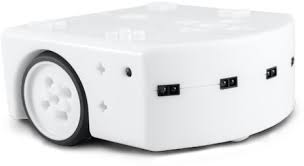
\includegraphics[scale=0.6]{res/thymio.jpg}
		\end{center}
	\end{figure}
	\section{Raspberry-Pi}
	\textbf{Description}
	\paragraph{}
	The Raspberry-Pi is a s single-board computer with wireless LAN and Bluetooth connectivity. It needs a micro USB power supply (2.1 A) in order to be plugged into a power-bank. It has 1GB RAM, 4 USB 2 ports, Full size HDMI, 100 base Ethernet and including a quad core 1.2GHz Broadcom BCM2837 64bit CPU.\\ \\
	\textbf{Data sheet} 
	\paragraph{}
	\url{https://www.raspberrypi.org/products/raspberry-pi-3-model-b/}
	\begin{figure}[H]
		\begin{center}
			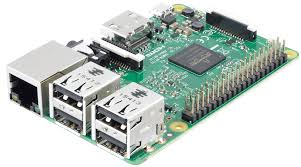
\includegraphics[scale=0.6]{res/raspberry.jpg}
		\end{center}
	\end{figure}
	\section{Raspberry-Pi Camera}
	\textbf{Description}
	\paragraph{}
	The Raspberry-Pi Camera delivers a 5MP resolution image, and 1080p HD video recording at 30 frame/second. It plugs into the Camera Serial Interface connector on the Raspberry-Pi. \\ \\
	\textbf{Data sheet} 
	\paragraph{}
	\url{https://uk.pi-supply.com/products/raspberry-pi-camera-board-v1-3-5mp-1080p?lang=fr}
	\begin{figure}[H]
		\begin{center}
			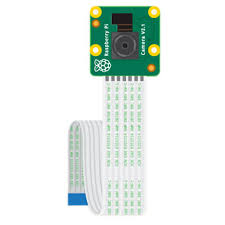
\includegraphics[scale=0.6]{res/camera.jpg}
		\end{center}
	\end{figure}
	\section{Power-bank}
	\textbf{Description}
	\paragraph{}
	For testing, we used RAVPower powerbank to power the Raspberry-Pi. It has 2A input which can charge the 6700 mAh portable charger. this feature guarantees that the Raspberry-Pi's services work correctly. \\ \\
	\textbf{Data sheet} 
	\paragraph{}
	\url{https://www.ravpower.com/p/Ravpower-6700mAh-Portable-Charger.html}
	\begin{figure}[H]
		\begin{center}
			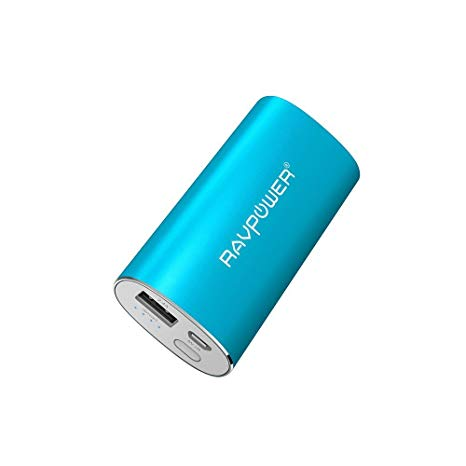
\includegraphics[scale=0.6]{res/power.jpg}
		\end{center}
	\end{figure}
\chapter{Conversion between pixels and centimeters}
\paragraph{}
In this section, we explain how we built the conversion system which permitted us to use the distances in pixels in the reality.
\paragraph{}
Firstly, we performed measurements to know the dimensions of objects in pixels and in centimeters depending on a certain distance from the camera. So we measured:
\begin{itemize}
	\item The real distance from the autonomous robot to the object (in centimeters).
	\item The real width of the object (in centimeters).
	\item The distance in pixels between the autonomous robot and the object.
	\item The width in pixels of the object.
\end{itemize}
\section{Nonlinear Regression}
	\paragraph{}
	The first table contains the equivalence between the real distance in centimeters and the one in pixels, between an object and the autonomous robot. The distance in pixels is the column X and the one in centimeters is in the column Y.
	\begin{figure}[H]
		\begin{center}
			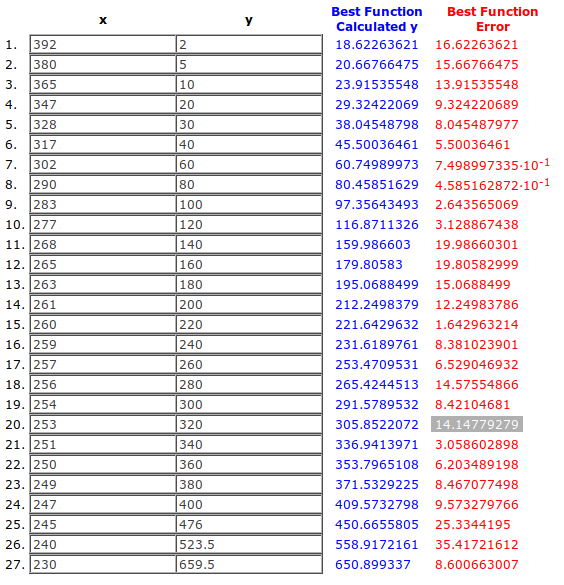
\includegraphics[scale=0.6]{res/reg2D.png}
			\caption{Equivalence pixels-centimeters for the distance between the robot and the object}
		\end{center}
	\end{figure}
\paragraph{}
We performed a Nonlinear Regression on the data to obtain an equation with the distance in pixels as entry and the distance in centimeters as a result.

\paragraph{}
We can see in the column "Best function calculated Y" the real distance estimated by the equation, knowing the distance in pixels. And in the column "Best function error", the difference between the distance in centimeters we have measured and the one estimated by the equation. The biggest error is estimated at 14.15 with X=253 and Y=320. 
\section{Multiple Polynomial Regression}
In the second table, we have 2 entries: The width in pixels of that object in pixels (X1), and the real distance between the object and the autonomous robot (X2). The third column represents the output which is the real width of the object.
\begin{figure}[H]
	\begin{center}
		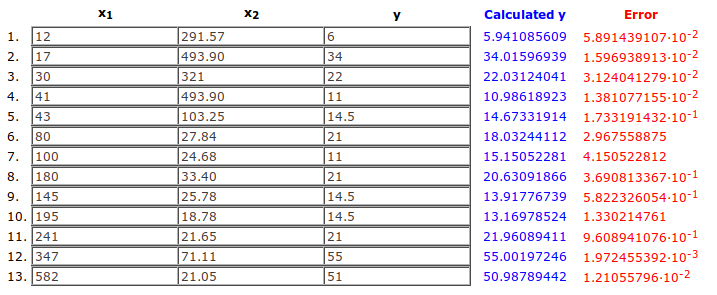
\includegraphics[scale=0.6]{res/reg3D.png}
	\end{center}
\end{figure} 

\paragraph{}
We performed a Multiple Polynomial Regression on the data to obtain an equation which estimates the real width of the object.

\paragraph{}
We can see in the column "Calculated Y" the real width estimated by the equation. And in the column "Error", the difference between the real width of the object we have measured and the one estimated by the equation. The biggest error is estimated at 4.15 with X1=100, X2= 24.36 and Y=11.

\paragraph{}
For both Nonlinear Regression and Multiple Polynomial Regression, the error remains acceptable because it is in centimeters and we remind that our goal is only to build roughly the environment. So, we do not need that precision of estimation.
	\chapter{3D Object recognition for Deep Learning}

	\paragraph{}
	Our works may improved by considering a database with 3D models, instead of a 2D ones. Than, if the database is large, the recognition process takes a long time to execute. Because in our strategy, we try to match the picture taken by the autonomous robot with each element of the database. Using deep learning for 3D object recognition may be a suitable solution to this issue.
	
	\paragraph{}
	In this case, we have begun to work on 3D object recognition. We developed a \textbf{View Generator} which reads a mesh file and performs a 2D projections of the 3D model at different views.
	
	\begin{figure}[H]
		\begin{center}
			\includegraphics[scale=0.6]{res/multiviews.png}
			\caption{Multi-views generation of a 3D model}
		\end{center}
	\end{figure} 
\paragraph{}
After generating the multi-views of different objects, the result consists of the new database on which the learning phase should stand. 
\end{document}
